\documentclass[preprint, 3p,
authoryear]{elsarticle} %review=doublespace preprint=single 5p=2 column
%%% Begin My package additions %%%%%%%%%%%%%%%%%%%

\usepackage[hyphens]{url}

  \journal{GEOG 712 Reproducible Research Workflow with GitHub and
R} % Sets Journal name

\usepackage{graphicx}
%%%%%%%%%%%%%%%% end my additions to header

\usepackage[T1]{fontenc}
\usepackage{lmodern}
\usepackage{amssymb,amsmath}
% TODO: Currently lineno needs to be loaded after amsmath because of conflict
% https://github.com/latex-lineno/lineno/issues/5
\usepackage{lineno} % add
\usepackage{ifxetex,ifluatex}
\usepackage{fixltx2e} % provides \textsubscript
% use upquote if available, for straight quotes in verbatim environments
\IfFileExists{upquote.sty}{\usepackage{upquote}}{}
\ifnum 0\ifxetex 1\fi\ifluatex 1\fi=0 % if pdftex
  \usepackage[utf8]{inputenc}
\else % if luatex or xelatex
  \usepackage{fontspec}
  \ifxetex
    \usepackage{xltxtra,xunicode}
  \fi
  \defaultfontfeatures{Mapping=tex-text,Scale=MatchLowercase}
  \newcommand{\euro}{€}
\fi
% use microtype if available
\IfFileExists{microtype.sty}{\usepackage{microtype}}{}
\usepackage[]{natbib}
\bibliographystyle{elsarticle-harv}

\usepackage{graphicx}
\ifxetex
  \usepackage[setpagesize=false, % page size defined by xetex
              unicode=false, % unicode breaks when used with xetex
              xetex]{hyperref}
\else
  \usepackage[unicode=true]{hyperref}
\fi
\hypersetup{breaklinks=true,
            bookmarks=true,
            pdfauthor={},
            pdftitle={Food Deserts or Food Oases? Predicting Grocery Store Locations in Hamilton, Ontario},
            colorlinks=false,
            urlcolor=blue,
            linkcolor=magenta,
            pdfborder={0 0 0}}

\setcounter{secnumdepth}{5}
% Pandoc toggle for numbering sections (defaults to be off)


% tightlist command for lists without linebreak
\providecommand{\tightlist}{%
  \setlength{\itemsep}{0pt}\setlength{\parskip}{0pt}}




\usepackage{tabularx}
\usepackage{float}
\floatplacement{figure}{H}
\usepackage{bm}




\begin{document}


\begin{frontmatter}

  \title{Food Deserts or Food Oases? Predicting Grocery Store Locations
in Hamilton, Ontario}
    \author[sees]{Zehui Yin%
  \corref{cor1}%
  }
   \ead{yinz39@mcmaster.ca} 
      \affiliation[sees]{
    organization={School of Earth, Environment \& Society, McMaster
University},addressline={1280 Main Street
West},city={Hamilton},postcode={L8S
4K1},state={Ontario},country={Canada},}
    \cortext[cor1]{Corresponding author}
  
  \begin{abstract}
  Grocery stores play a crucial role, especially for urban residents, as
  they provide essential daily food supplies. The locations of grocery
  stores are not randomly chosen but are the result of detailed
  decision-making processes by grocery companies. Understanding the
  locations these grocers choose to establish themselves is important
  for public health and urban planning, as geographic access to grocery
  stores impacts personal health. In this paper, I utilize open data to
  examine grocery store locations in Hamilton, Ontario, as a case study.
  A zero-inflated negative binomial regression model with spatial lagged
  terms is fitted and estimated using maximum likelihood methods. I
  identified noticeable spatial patterns in grocery store locations.
  Grocery stores tend to cluster in nearby dissemination areas, but when
  there are too many grocery stores, they tend to disperse. The number
  of grocery stores is also significantly associated with population
  density, dissemination area size, the percentage of residents who do
  not speak an official language at home, those living in single
  detached houses, and the distance to Hamilton downtown.
  \end{abstract}
    \begin{keyword}
    Grocery stores \sep Food environments \sep 
    Hamilton
  \end{keyword}
  
 \end{frontmatter}

\section{Introduction and Background}\label{introduction-and-background}

Food is a necessity for human beings. In urban areas or large cities,
residents typically rely on grocery stores for their daily food needs.
Geographic access to grocery stores and affordable food plays an
important role in promoting a healthy diet and has implications for
personal health
\citep{caspi2012relationship, minaker2016retail, kirkpatrick2014dietary}.
The ease of accessing grocery stores and obtaining the needed food is
thus an important topic for both public health and urban planning.

There is extensive literature on food access that examines this topic
\citep{christian2012using, widener2015spatiotemporal, farber2014temporal, widener2017changes}.
These analyses mostly focus on the demand side, where consumers navigate
and choose which retailers to purchase from. However, a gap exists in
studying how retailers choose the locations of their stores to serve the
market or the demand.

In this paper, I utilize open-source data from the 2021 Canadian Census
\citep{census} and OpenStreetMap \citep{osm} to examine the spatial
pattern of grocery store locations, using Hamilton, Ontario, as a case
study. The research question for this paper is: What areas in Hamilton
have more or fewer grocery stores compared to other areas?

\section{Data and Methods}\label{data-and-methods}

\subsection{Study Area}\label{study-area}

My study area is the City of Hamilton, located on the west side of Lake
Ontario in the province of Ontario. It has a population of 569353
according to the 2021 Canadian census \citep{census}. The Niagara
Escarpment runs through the middle of the city, dividing it into two
parts. Figure \ref{fig:study_area} below shows the study area.

\begin{figure}
\centering
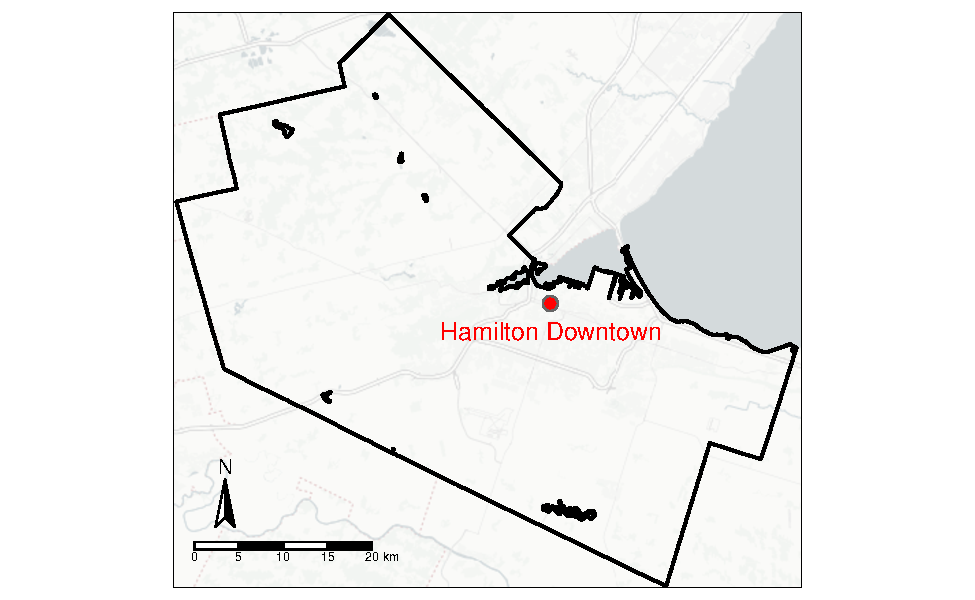
\includegraphics{grocery_store_hamilton_files/figure-latex/unnamed-chunk-4-1.pdf}
\caption{\label{fig:study_area}Study Area: Hamilton, Ontario}
\end{figure}

\subsection{Data Sources}\label{data-sources}

I utilize three data sources in this paper, as shown in the Table
\ref{tab:data_source} below. I gathered grocery store locations in
Hamilton from OpenStreetMap \citep{osm} via the Overpass API
\citep{overpass}. The Hamilton Street Railway (HSR) Fall 2024 GTFS
static data were downloaded from Open Hamilton \citep{hsr_gtfs}. The
dissemination area (DA) spatial data and 2021 Canadian census variables
were obtained from \citet{census} through the cancensus package in R
\citep{cancensus}.

\begin{table}[h]
\centering
\begin{footnotesize}
\begin{tabularx}{\textwidth}{XXll}
\hline
Name                                           & Source              & URL                                             & Accessed Date \\
\hline
Grocery Stores in Hamilton                     & \cite{osm}          & \url{https://overpass-turbo.eu/index.html}      & 2024-10-04    \\
HSR Fall 2024 GTFS Static                      & \cite{hsr_gtfs}     & \url{https://opendata.hamilton.ca/GTFS-Static/} & 2024-10-04    \\
Dissemination Area and Census Data in Hamilton & \cite{census}       & \url{https://censusmapper.ca/api}               & 2024-11-16    \\
\hline
\end{tabularx}
\caption{\label{tab:data_source}Data Sources}
\end{footnotesize}
\end{table}

To facilitate reproducibility and open science, all the data used in
this paper have been packaged into an R package \citep{geog712package},
which is hosted on GitHub. You can access it at
\url{https://github.com/zehuiyin/geog712package}.

\subsection{Methodology}\label{methodology}

The grocery store locations in Hamilton were intersected and aggregated
to the census dissemination areas. The dependent variable of interest is
the count of grocery stores in each dissemination area in Hamilton.
There are 891 dissemination areas in Hamilton; however, due to data
missingness, only 876 of them are used in the regression analysis. A
considerable portion of the dissemination areas in our sample do not
contain any grocery stores. Therefore, standard count models such as
Poisson regression would be invalid due to the excessive zero values. To
model this variable of interest, I fit a hurdle model and a
zero-inflated negative binomial regression model with spatially lagged
dependent variables.

The zero-inflated negative binomial regression model follows Equations
\ref{eq:1} and \ref{eq:2} below \citep{zinb}. The variable specification
in the hurdle model is exactly the same as in the zero-inflated negative
binomial regression model. The hurdle model is set up with the zero
component as a binomial logit model and the count component as a
truncated negative binomial logit model. I decided to use negative
binomial regression instead of Poisson regression because the count
distribution is highly skewed, making it unlikely that the mean and
variance would be the same for my variable of interest. Additionally,
due to the large number of zeros in my sample, the zero-inflated
regression is preferred, as it can generate zero values from two
sources, unlike the hurdle model, which generates zeros from only one
source.

\begin{equation}
\label{eq:1}
Pr(GroceryStore_i=j) = \begin{cases}
       \pi_i + (1-\pi_i)g(GroceryStore_i=0) &\quad\text{if } j=0\\
       (1-\pi_i)g(GroceryStore_i) &\quad\text{if } j>0
     \end{cases}
\end{equation}

\begin{equation}
\label{eq:2}
\begin{aligned}
logit(\pi) &= \rho \mathbf{W} GroceryStore + \tilde{\mathbf{x}} \tilde{\boldsymbol{\beta}} \\
\log\{E[g(GroceryStore)]\} &= \rho \mathbf{W} GroceryStore + \mathbf{x} \boldsymbol{\beta} \\
g(GroceryStore_i) &\text{ is the negative binomial distribution} \\
\mathbf{W} &\text{: a row-normalized queen contiguity matrix}
\end{aligned}
\end{equation}

\section{Results}\label{results}

\subsection{Descriptive Statistics}\label{descriptive-statistics}

Based on the bar chart in Figure \ref{fig:dep}, the distribution of the
number of grocery stores in dissemination areas in Hamilton is highly
skewed, with a large number of dissemination areas having no grocery
stores. According to Figure \ref{fig:descriptive}, most grocery stores
are located near the centre of Hamilton, within the Niagara Escarpment.
There are also some dissemination areas at the edge of the city with
grocery stores. In the right plot, the number of HSR bus stops per
square kilometre is classified into three categories: low (0 to 50th
percentile), middle (50th to 75th percentile), and high (75th to 100th
percentile). The area with the highest transit service is also in the
centre of Hamilton. Beyond the Niagara Escarpment, there are few transit
stops.

\begin{figure}

{\centering 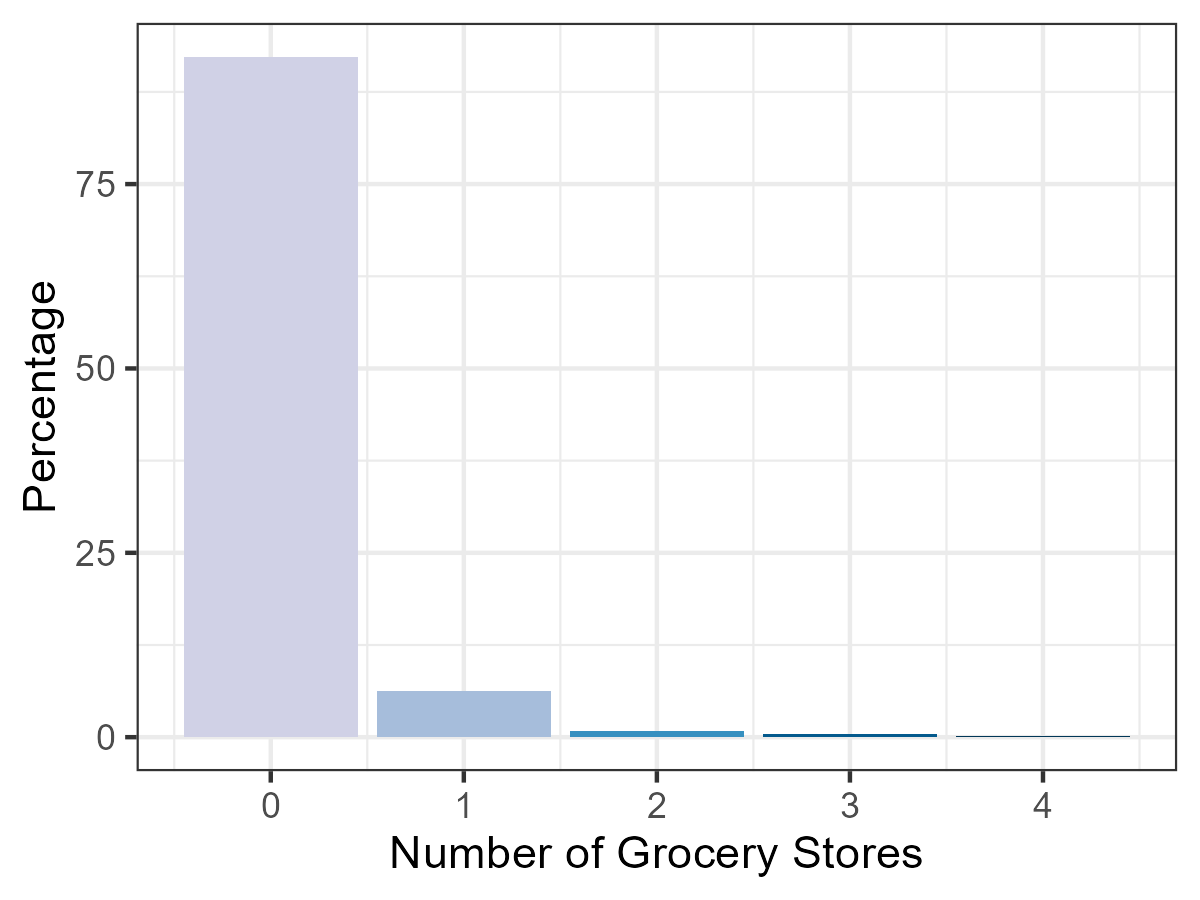
\includegraphics[width=4in,height=3in]{./images/dep} 

}

\caption{\label{fig:dep}Number of Grocery Stores in Dissemination Areas in Hamilton}\label{fig:unnamed-chunk-10}
\end{figure}

\begin{figure}

{\centering 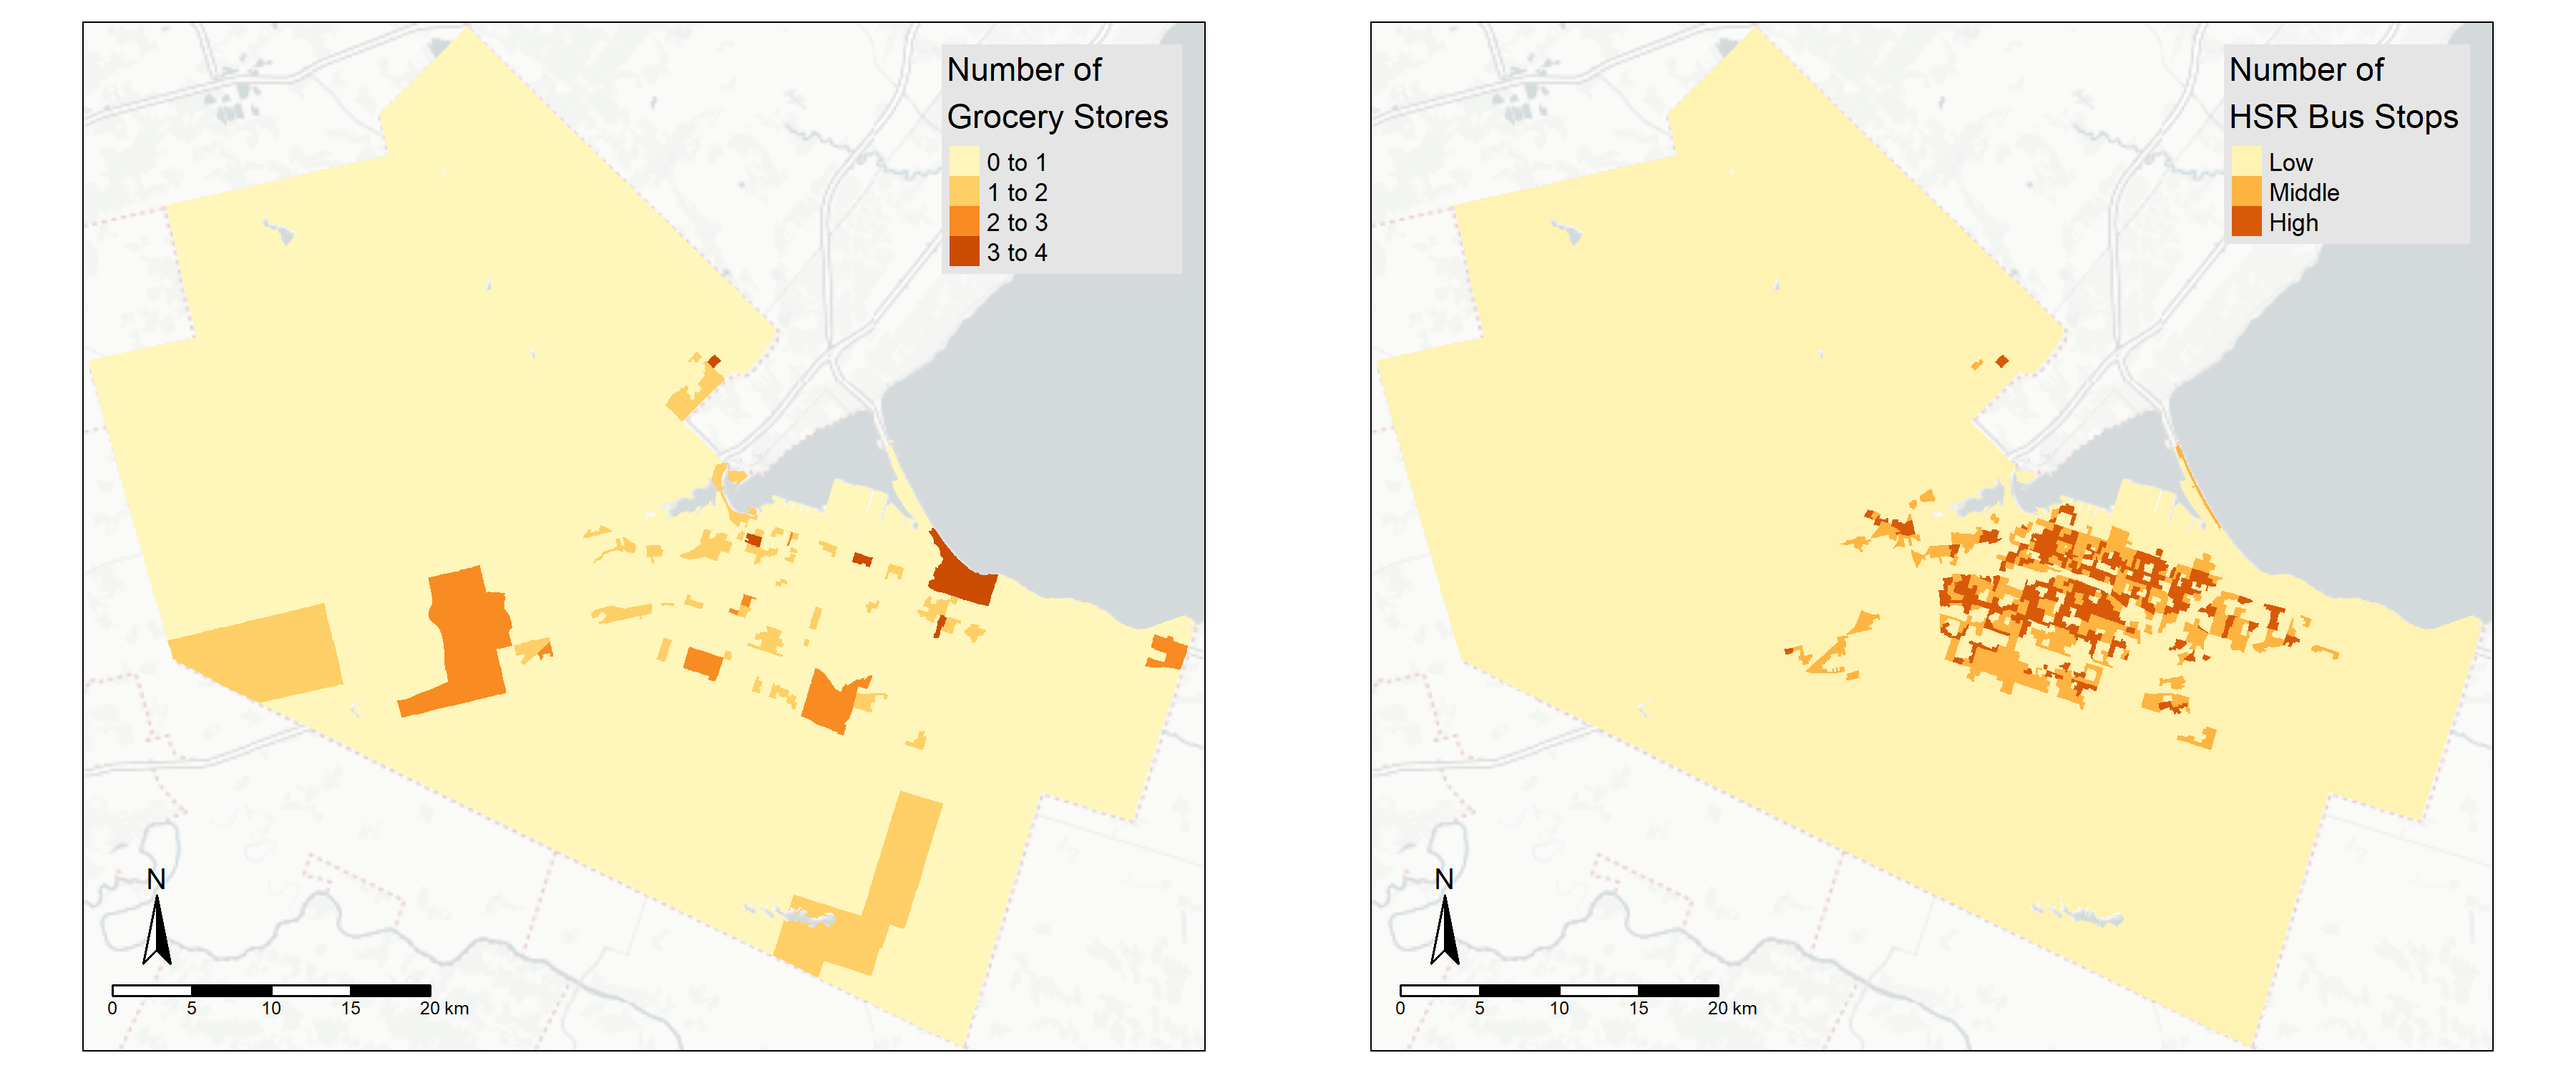
\includegraphics[width=6in,height=2.5in]{./images/descriptive} 

}

\caption{\label{fig:descriptive}Number of Grocery Stores (left) and HSR Bus Stops (right) at Dissemination Areas in Hamilton, Ontario}\label{fig:unnamed-chunk-13}
\end{figure}

\subsection{Regression Results}\label{regression-results}

The regressions are estimated using the maximum likelihood method with
the R package pscl \citep{pscl}. The hurdle model has a McFadden pseudo
\(R^2\) of 0.15, while the zero-inflated negative binomial regression
model has a McFadden pseudo \(R^2\) of 0.17. A pseudo \(R^2\) around
0.17 is relatively small but common in this type of model and in social
science. Table \ref{tab:regression_results} below presents the
regression results.

\begin{table}
\begin{center}
\begin{footnotesize}
\begin{tabular}{l c c}
\hline
 & Hurdle model & Zero-inflated model \\
\hline
Count model: Spatial lag of grocery store count                               & $-2.05$      & $-2.99^{***}$   \\
                                                                              & $(2.37)$     & $(0.84)$        \\
Count model: Percentage of population aged below 24 years old                 & $-0.06$      & $0.03$          \\
                                                                              & $(0.11)$     & $(0.04)$        \\
Count model: Percentage of population aged above 65 years old                 & $-0.02$      & $0.02$          \\
                                                                              & $(0.05)$     & $(0.02)$        \\
Count model: Percentage of population don't know official language            & $-0.11$      & $-0.03$         \\
                                                                              & $(0.26)$     & $(0.10)$        \\
Count model: Percentage of population don't speak official language at home   & $0.08$       & $0.17^{**}$     \\
                                                                              & $(0.12)$     & $(0.06)$        \\
Count model: Percentage of population live in single detached houses          & $-0.01$      & $-0.01^{\cdot}$ \\
                                                                              & $(0.02)$     & $(0.01)$        \\
Count model: Percentage of population have annual total income less than 40K  & $0.02$       & $-0.03$         \\
                                                                              & $(0.09)$     & $(0.03)$        \\
Count model: Percentage of population have annual total income more than 100K & $-0.04$      & $-0.02$         \\
                                                                              & $(0.10)$     & $(0.04)$        \\
Count model: Percentage of population that are married or live in common-law  & $0.02$       & $0.03$          \\
                                                                              & $(0.08)$     & $(0.03)$        \\
Count model: Natural log of (population density + 1)                          & $-0.59$      & $-0.38^{*}$     \\
                                                                              & $(0.37)$     & $(0.17)$        \\
Count model: Natural log of distance from DA centroid to Hamilton downtown    & $-0.25$      & $-0.50^{**}$    \\
                                                                              & $(0.43)$     & $(0.19)$        \\
Zero model: Spatial lag of grocery store count                                & $0.02$       & $-8.62^{*}$     \\
                                                                              & $(0.58)$     & $(3.38)$        \\
Zero model: Percentage of population don't speak official language at home    & $0.10^{**}$  & $0.14$          \\
                                                                              & $(0.03)$     & $(0.11)$        \\
Zero model: Percentage of population that are married or live in common-law   & $-0.04^{*}$  & $0.11$          \\
                                                                              & $(0.02)$     & $(0.07)$        \\
Zero model: Natural log of (population density + 1)                           & $0.73^{*}$   & $-1.71^{*}$     \\
                                                                              & $(0.29)$     & $(0.74)$        \\
Zero model: Number of HSR bus stops (50-75 percentile)                        & $2.15^{***}$ & $-2.73^{***}$   \\
                                                                              & $(0.43)$     & $(0.72)$        \\
Zero model: Number of HSR bus stops (75-100 percentile)                       & $1.55^{**}$  & $-1.50^{*}$     \\
                                                                              & $(0.49)$     & $(0.74)$        \\
Zero model: Natural log of area size in square kilometres                     & $1.39^{***}$ & $-2.36^{**}$    \\
                                                                              & $(0.29)$     & $(0.76)$        \\
\hline
AIC                                                                           & $522.36$     & $508.91$        \\
Log Likelihood                                                                & $-240.18$    & $-233.45$       \\
Num. obs.                                                                     & $876$        & $876$           \\
\hline
\multicolumn{3}{l}{\tiny{$^{***}p<0.001$; $^{**}p<0.01$; $^{*}p<0.05$; $^{\cdot}p<0.1$}}
\end{tabular}
\end{footnotesize}
\caption{Regression results}
\label{tab:regression_results}
\end{center}
\end{table}

Both models have the same variable specification. Almost all the
variables in the hurdle model's zero component are significant, while no
variables in its count component are significant. Meanwhile, the
zero-inflated negative binomial regression model has significant
variables in both the zero and count components. Considering that the
pseudo \(R^2\) for the zero-inflated model is also higher than that of
the hurdle model, the zero-inflated model provides a better fit compared
to the hurdle model. Therefore, in the following sections, I will focus
on interpreting the zero-inflated model.

The zero component in the zero-inflated negative binomial regression is
a binary logit model predicting the probability of zero inflation. Thus,
a positive coefficient indicates that the variable is contributing
positively or increasing the probability of a specific dissemination
area having zero grocery stores, while a negative coefficient suggests
the opposite. The count component in the model is a negative binomial
regression predicting the number of grocery stores in a dissemination
area. Therefore, a positive coefficient indicates that an increase in
the variable's value is associated with an increase in the expected
count of grocery stores in that specific dissemination area.

The spatial lagged term of grocery store counts is a significant
negative predictor in both components of the model. This indicates that
a higher number of grocery stores in neighbouring dissemination areas
would lower the number of grocery stores in the specific dissemination
area, while it would reduce the probability that the specific
dissemination area would have zero grocery stores. Thus, it has a
non-monotonic effect on grocery store counts. Similarly, the natural log
of population density plus one also has a significant negative effect on
both components of the model. Additionally, the percentage of the
population that does not speak an official language at home is
significantly positively associated with more grocery stores. The
percentage of the population living in single detached houses and the
natural log of distance from the dissemination area centroid to Hamilton
downtown both decrease the expected number of grocery stores in the
dissemination area.

Regarding the zero component, the 50-75 percentile and 75-100 percentile
in the number of HSR bus stops are significantly associated with a lower
probability of having zero grocery stores compared to the reference
category (0-50 percentile). Meanwhile, as the area size of the
dissemination area increases, the probability of having zero grocery
stores decreases.

\begin{figure}

{\centering 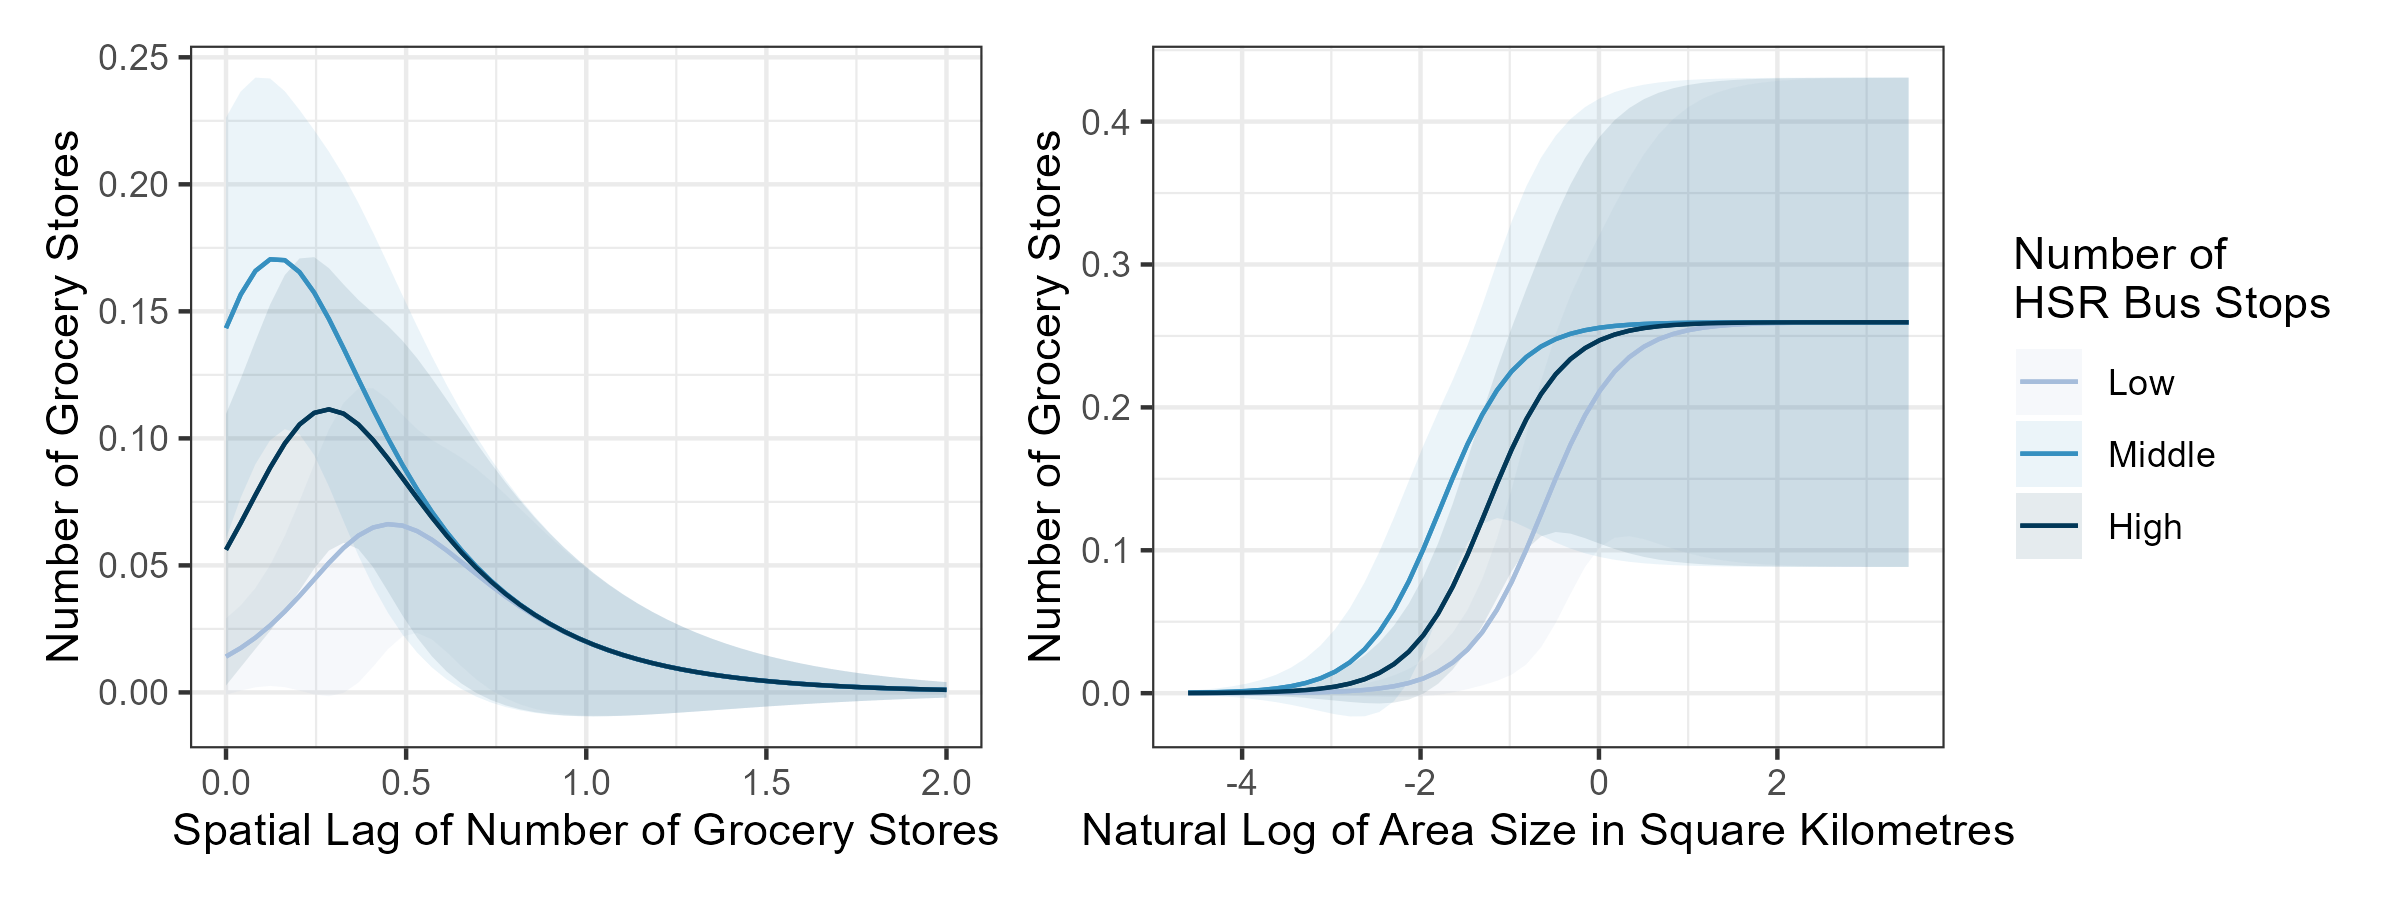
\includegraphics[width=6.3in,height=2.1in]{./images/margin} 

}

\caption{\label{fig:margin}Conditional Prediction Plot for the Zero-inflated Negative Binomial Regression Model}\label{fig:unnamed-chunk-18}
\end{figure}

Figure \ref{fig:margin} above shows the prediction plot for the
zero-inflated model. The spatial lagged term and population density
exhibit non-monotonic effects on grocery store counts. As the number of
grocery stores in neighboring dissemination areas increases, holding all
else constant, the expected grocery store count first increases and then
decreases. Similarly, as the population density in the dissemination
area increases, the expected grocery store count first increases and
then decreases.

Dissemination areas with the number of HSR bus stops in the 50-75th
percentile have the highest average grocery store count compared to the
other two levels. It is not surprising that dissemination areas with the
lowest transit access have the lowest expected grocery store count.

The model predicts that as the size of the dissemination area increases
from approximately 0.14 to 1 square kilometres, holding all else
constant, there would be an expected increase in the grocery store
count. However, as the area size further increases or decreases, the
grocery store count does not change significantly.

\section{Discussion and Conclusion}\label{discussion-and-conclusion}

Based on the regression results, I found that grocery stores in Hamilton
tend to be located in census dissemination areas where the neighbouring
dissemination areas have, on average, 0.4 grocery stores. If
neighbouring dissemination areas have more or fewer grocery stores on
average, the expected number of grocery stores in that dissemination
area decreases. An excess of grocery stores in nearby dissemination
areas likely saturates the market, reducing the demand for new stores.
Conversely, a lack of grocery stores in neighbouring areas might
indicate an overall low demand in the local geography, which is also
associated with a lower expected number of grocery stores in the
specific census dissemination area. Additionally, evidence indicates
that grocery stores tend to be located in dissemination areas with
moderate population densities, approximately 2980.96 per square
kilometre. Low population density suggests a smaller market demand,
while high population density might be associated with high land prices,
constituting a high fixed cost for operating a grocery store.

As the dissemination area size increases to about 1 square kilometre, it
exhibits the highest predicted number of grocery stores, indicating that
a sufficient dissemination area size is needed for operating a grocery
store. However, further increases in dissemination area size do not
significantly impact the number of grocery stores, likely because many
large dissemination areas in Hamilton are suburban areas around the
city's edge with no grocery stores. The number of HSR bus stops is
positively associated with the presence of grocery stores in a specific
dissemination area, indicating that areas with better transit access are
more likely to have grocery stores. Better transit access increases the
potential catchment area of a grocery store, attracting more customers.

I also found that grocery stores tend to be located in areas with a
higher percentage of the population that does not speak an official
language at home, while the presence of single detached houses and the
distance to Hamilton downtown are negatively associated with the
presence of grocery stores. Non-English or French-speaking residents in
Hamilton are more likely to be newcomers with limited mobility options
and might choose to live in areas where they can easily access food.
Meanwhile, the areas with many single detached houses and those far from
Hamilton downtown might be residential zones where commercial activity
is limited due to institutional factors.

In this paper, I utilized open data to examine the spatial locations of
grocery stores in Hamilton, Ontario. I found noticeable spatial patterns
in grocery store locations. Grocery stores tend to cluster together in
nearby dissemination areas, but when there are too many grocery stores,
they are more likely to disperse. The number of grocery stores is also
significantly associated with population density, dissemination area
size, the percentage of residents who do not speak an official language
at home and live in single detached houses, and the distance to Hamilton
downtown.

There are some limitations in this paper. Euclidean distances were used
to measure the distance from the dissemination area centroid to Hamilton
downtown, but a network distance could provide more accurate
measurements. Additionally, distances could be computed using more
sample points within a dissemination area instead of relying solely on
the centroid. The model is based on a cross-sectional dataset, so no
causal relationships can be concluded in this context. Utilizing a panel
dataset with several years of census data could better shed light on the
causal relationships between these variables and the number of grocery
stores. Furthermore, the analysis treated all grocery stores equally,
regardless of their physical size or sales volume. Using additional data
sources to better capture the size of these businesses could help
improve the model.

\pagebreak

\renewcommand\refname{References}
\bibliography{mybibfile.bib}


\end{document}
